\documentclass[]{article}
\usepackage{graphicx}
\begin{document}

\begin{center}
    \vspace*{1cm}

    \textbf{Question 2.}

    \vspace{0.5cm}
     Algorithms Assignment 1

    \vspace{0.15cm}

    \textbf{Faaiq Bilal} \\ 
    \textbf{23100104}
         
\end{center}

\section{Part a}

$ n^2 = 3.6 \times 10^{13} $ \\
$ n = \sqrt{3.6 \times 10^{13}}   $ \\
$ n = 6000000 $ 

\section{Part b}
$ n^3 = 3.6 \times 10^{13}$ \\
$ n = \sqrt[3]{3.6 \times 10^{13}} $ \\
$ n = 33019.27 $ \\
Assuming integer n (if this is conditional on our n) $ \Longrightarrow 33019 $ 

\section{Part c}
$ 100 n^2 = 3.6 \times 10^{13}$ \\
$ n^2 = 3.6 \times 10^{11}$ \\
$ n = 600000 $ 

\section{Part d}
It is not possible to generate a solution for $ n \log{n}$. We can use a graphical solution instead. \\ \\ 
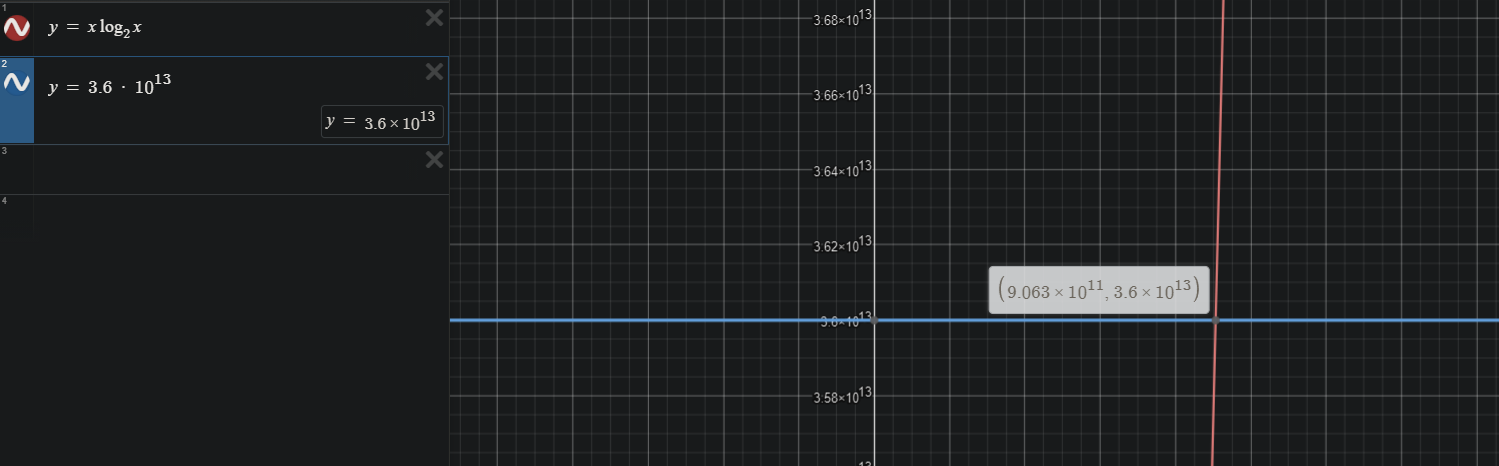
\includegraphics[scale=0.5]{Screenshot_14.png}
\\ This gives us $ n = 9.063 \times 10^{11} $ \\

\section{Part e}
$ 2^n = 3.6 \times 10^{13} $ \\
$ n = \log_2 (3.6 \times 10^{13}) $ \\
$ n = 45.03 $ \\
Assuming integer n (if this is conditional on our n)$ n = 45 $ 

\section{Part f}
$ 2^{2^n} = 3.6 \times 10^{13} $ \\
Applying logarithm of base 2 to simplify on both sides \\
$ 2^n = 45.03 $ \\
Applying logarithm of base 2 to simplify on both sides \\
$ n = 5.4929 $ \\
Assuming integer n (if this is conditional on our n)$ n = 5 $ 

\end{document}